\section{Methodology}

We intend to utilize the following methods:
\begin{itemize}
    \item[--] Exploratory analysis
    \item[--] Regression, https://www.alchemer.com/resources/blog/regression-analysis/
    \item[--] ARIMA, https://www.machinelearningplus.com/time-series/arima-model-time-series-forecasting-python/
    \item[--] LSTM --- Tensorflow
    \end{itemize}

\subsection{Data gathering}
In order to analyze data connected to salmon price, we first need to gather this data. 
The main data point is the price of salmon. There are several sources for this data, but we utilized the data from the NASDAQ salmon exchange.
The reason for this being a combination of the accessibility of the data, and the fact that the NASDAQ salmon exchange (NQSALMON)
uses a weighted average for the salmon price, gathered from a spectrum of salmon exporters and it is therefore the best source of meaningful data.
Another reason for using the NASDAQ salmon exchange is that the data is updated weekly with no missing values for the entire time frame.
We downloaded data from March 2013 through December 2022, for a total of 507 data points. This was our base for the independent factors.

The next step was to gather data from the other relevant factors for our analysis. 


\subsection{Exploratory analysis}

\subsection{ARIMA and SARIMAX}

As explained in~\ref{SeasonalityTheory} on page~\pageref{SeasonalityTheory}, one of the prerequisites for the ARIMA model is that the data is stationary. This can be done either by analysing the time-series itself and noticing the variance and trend, or by using the Augmented Dickey-Fuller test. 
After this is done, the next step will be to find the optimal parameters for the ARIMA model. This is usually done by looking at the ACF and PACF plots. 
When the optimal parameters are found, the model can be fitted and used to predict future values. \parencite{hyndman_athanasopoulos_2021}

\subsubsection{Determening stationarity}
The Augmented Dickey-Fuller test is a statistical test that can be used to determine stationarity. The null hypothesis of the test is that the time-series is non-stationary. If the p-value is less than the significance level, the null hypothesis is rejected and the time-series is expected to be stationary.
Using the Augmented Dickey-Fuller test on the Salmon Price data, we get a p-value of 0.05651, this means that we cannot reject the null hypothesis at a 95\% confidence level. The data is therefore not stationary.~\parencite{Dickey_Fuller1979}

In order to better understand why the data is not stationary, we can plot the data and look at the variance, trend and seasonality. This is done by decomposing the data into its components. We then get the following plot: 

\begin{figure}[H]
    \centering
    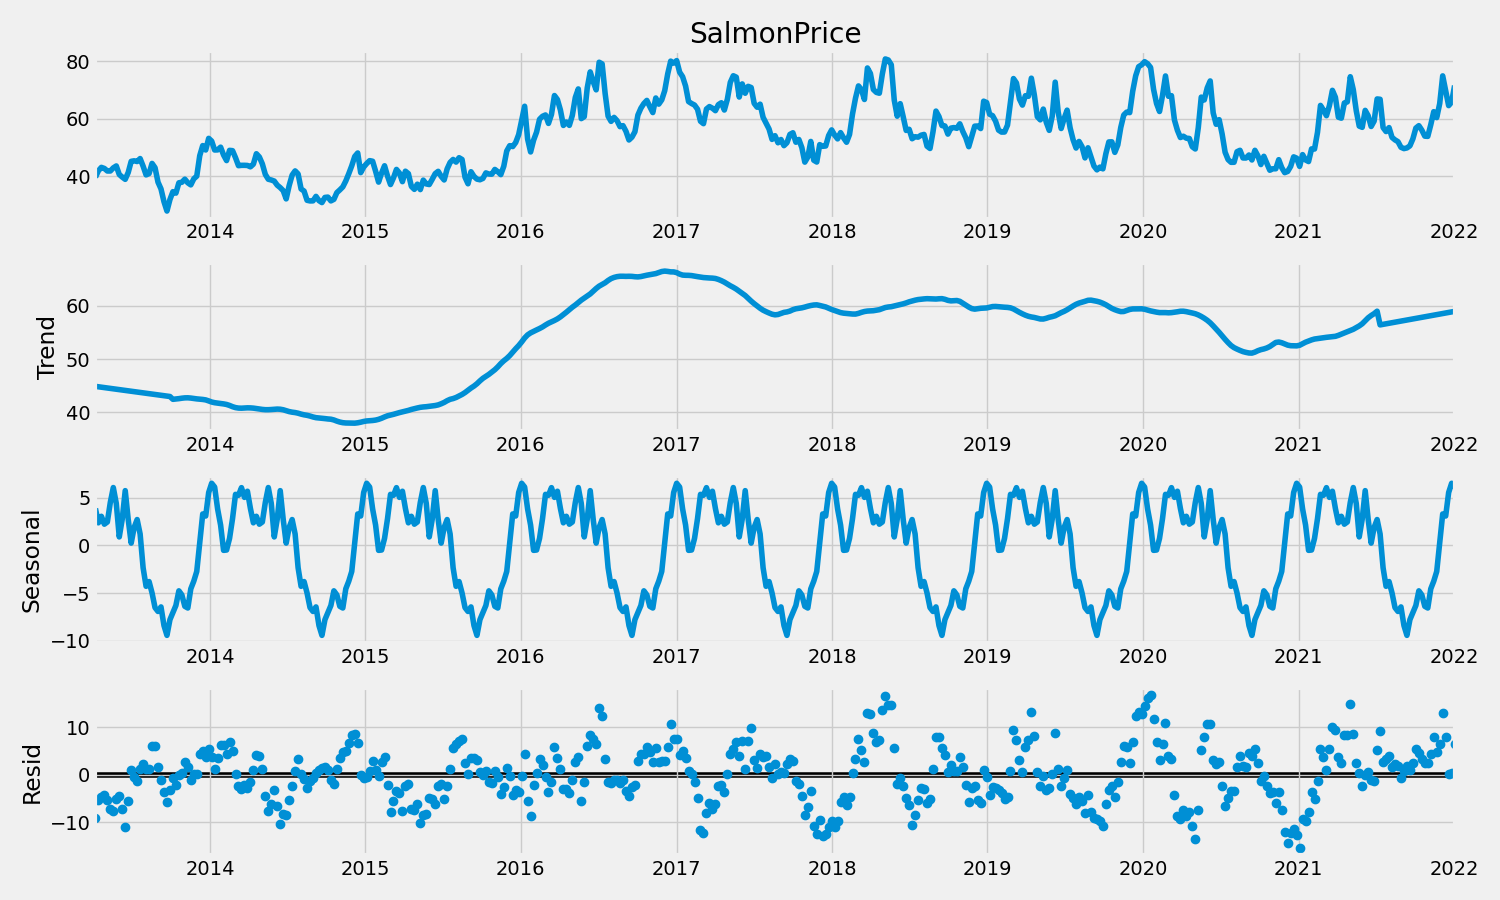
\includegraphics[width=0.8\textwidth]{data/Figures/ARIMA/Decomposition.png}
    \caption[Decomposition of the Salmon Price data]{Decomposition of the Salmon Price data.}\label{fig:Decomposition}
\end{figure}
Examining the decomposed data in Figure~\ref{fig:Decomposition} there are especially two things that stand out. The first is the trend, which is clearly increasing. The second is the seasonality, there is a clear yearly seasonal trend where the price is higher in the summer months before decreasing during the autumn and reaching a low in the winter. From this we can draw the same conclusion as the Augmented Dickey-Fuller test, the data is not stationary and needs differencing. In the ARIMA model, this will be done by setting $d$ to 1 or more. 

The exact number of differencing needed can be found either by using the ADF-test on the differenced data and looking for when the p-value is less than the critical value, or by looking at the autocorrelation plot and using rules set out by \textcite{nau_2019} to determine the number of differencing needed. 
\begin{figure}[H]
    \centering
    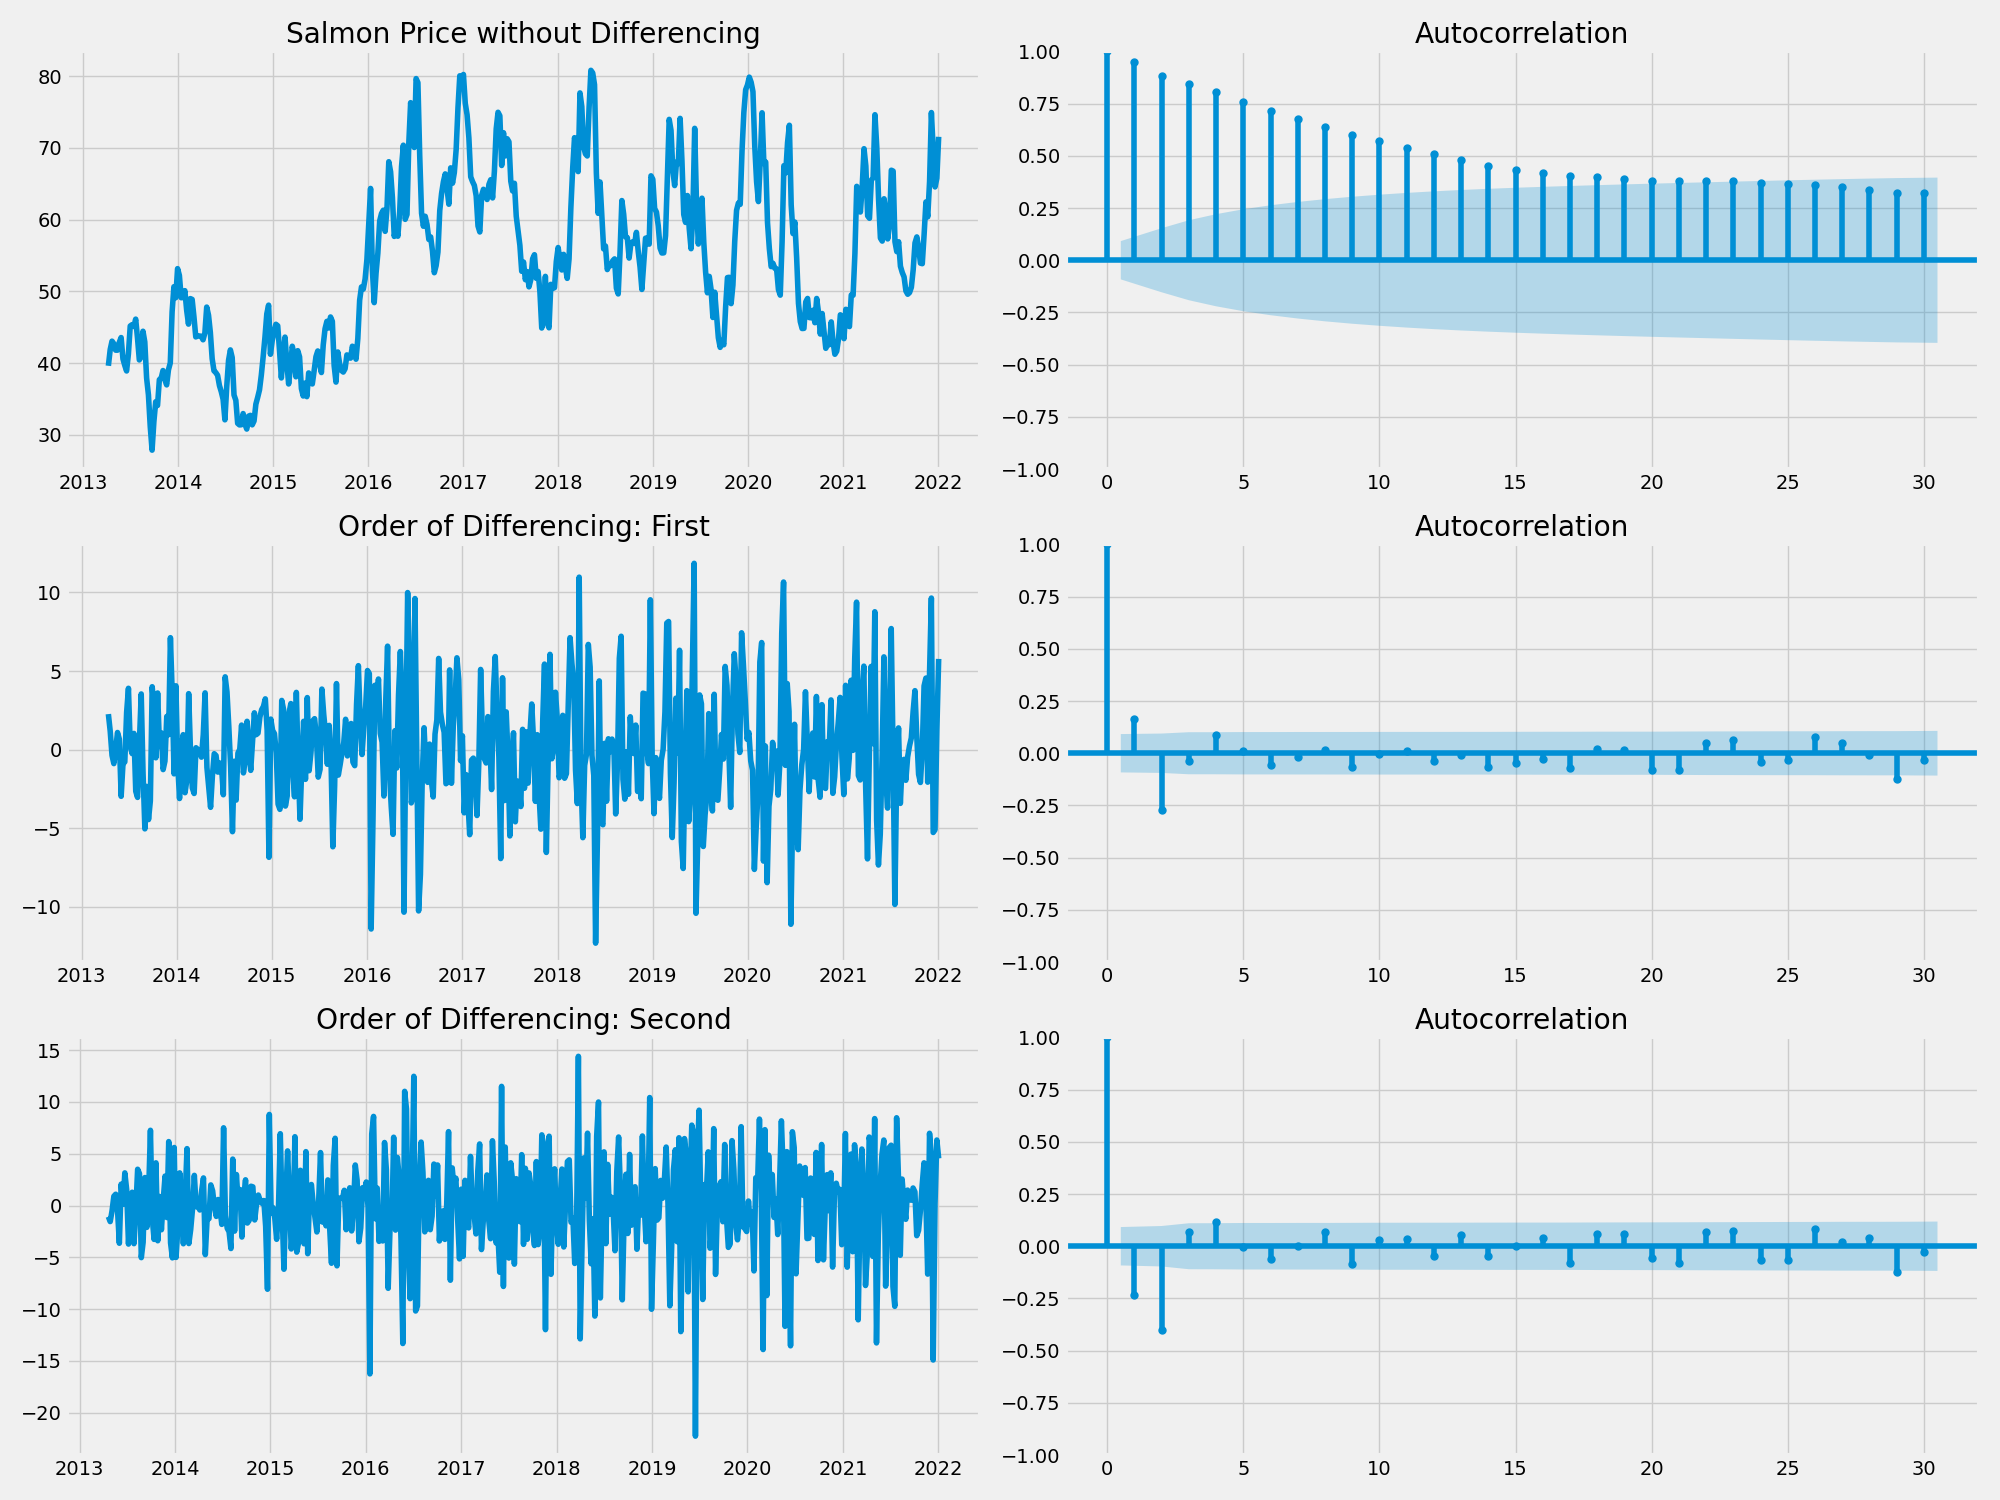
\includegraphics[width=0.8\textwidth]{data/Figures/ARIMA/Diff1_ACF_30.png}
    \caption[Different orders of differencing]{Different orders of differencing.}\label{fig:ACF_Differencing}
\end{figure}
Examining the trend and autocorrelation in Figure~\ref{fig:ACF_Differencing} we can see that the original data without differencing has both a clear trend and a slow decay in the autocorrelation plot with a high number of positive lags. Following the first rule from \textcite{nau_2019} we can conclude that the data needs at least one order of differencing.

After just a single order of differencing, the tends starts to flatten out and fluctuate around 0. The autocorrelation plot also drops sharply after the first lag, and is then quite small and patternless, this follows the second rule from \textcite{nau_2019} and will often be a sign that higher differencing is not needed. Running the Augmented Dickey-Fuller test on the differenced data, we get a p-value of 2.9705e-24, much lower than the critical value of 0.05. We can therefore reject the null hypothesis and conclude that the differenced data is stationary. 

With a second order of differencing, the trend seems to flatten even more, and the autocorrelation plot shows a sharp negative decline for the first and second lag, this may be a sign that the data is over-differenced. This is not optimal as over-differencing will lead to a loss of historical information and trends. It is therefore of utmost importance to find the order of differencing that both makes the data stationary and keeps the historical memory intact. Over-differencing is a common mistake when fitting non-stationary data to machine learning models, and can lead to the model not being able to capture the underlying trend.~\parencite{lopezde_prado2018}

A third way to determine the optimal number of differencing is, according to \textcite{nau_2019}, to look at the standard deviation of the plot at different orders of differencing. Following his rule number 3, the optimal number of differencing is the one where the standard deviation of the plot is the lowest. Examining Table~\ref{StdDevTable} we can see that the standard deviation of the data is lowest at the first order of differencing. After this the standard deviation increases, and there is no reason to believe any higher number of differencing will reduce the standard deviation. 

\begin{table}[h]
    \begin{center}
        \import{data/Figures/ARIMA/}{StdDevTable}
        \caption{\label{StdDevTable}Standard deviation of the differenced data.}
    \end{center}
\end{table}

We can therefore conclude that the optimal number of differencing should be 1.

\subsubsection{Autoregression and Moving Average}
The next step in a regular ARIMA model is to identify the optimal AR and MA terms needed to fit the model. This can be done by comparing different models by looking at the AIC and BIC values, but with larger models this would constitute an unnecessary use of computational power. The more efficient way to find the optimal terms is to look at the ACF and PACF plots of the differenced data and use the rules set out by \textcite{nau_2019} to determine the optimal terms. 
%data/Figures/ARIMA/DiffACF-PACF_30.png
\begin{figure}[H]
    \centering
    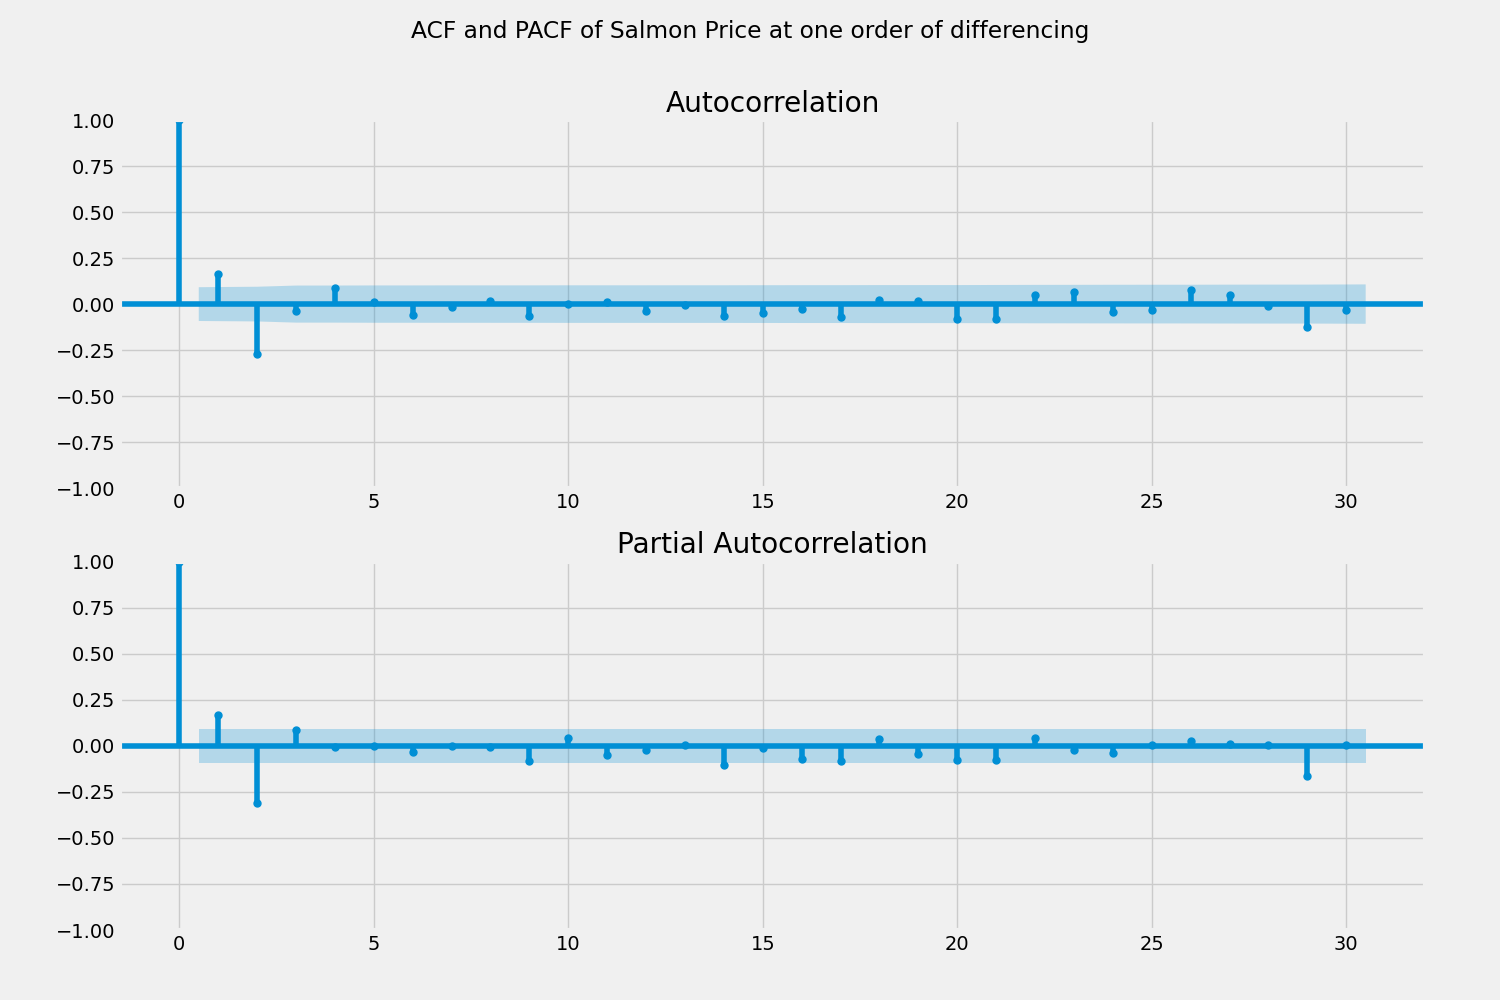
\includegraphics[width=0.8\textwidth]{data/Figures/ARIMA/DiffACF-PACF_30.png}
    \caption[ACF and PACF plots of the differenced data]{ACF and PACF plots of the differenced data.}\label{fig:ACF_PACF}
\end{figure}



\subsection{LSTM --- Tensorflow}